\setauthor{\secondauthor}

\section{Test Environment}
\subsection{Lighting Conditions}

\subsubsection{Shadow and Reflection Impact}
Lighting was also recognized as a key factor to ensure proper detection. Experiments were performed to identify how shadows cast by dart shafts and the person throwing created unstable contour shapes and periodic false motion areas. The problem was addressed by adding a light ring around the dartboard. This provided a more uniform light distribution on the dartboard surface while reducing directional shadows considerably.

Under this new lighting condition, contour detection was more stable during successive throws, especially around areas close to ring boundaries where small variations in lighting would normally cause variations in tip position. Errors observed under this new lighting condition were mainly due to calibration issues.


\subsection{Camera Setup}\label{subsec:eval_camera_setup}

\subsubsection{Distance, Angle, and FPS}\label{subsubsec:eval_camera_distance_angle_fps}
All evaluation runs were performed with the following camera configuration:

\begin{itemize}
	\item Webcam model: UGREEN Camera 4K
	\item Resolution: $1920 \times 1080$ (FHD)
	\item Effective frame rate during testing: 26 FPS
	\item Stream mode: RGB video
	\item Approximate field setup: camera angle $\approx 50^{\circ}$, camera distance $\approx 60\,\mathrm{cm}$
\end{itemize}

Other camera characteristics that were noted during the setup process were the image size, which was 2.07 MP and the aspect ratio, which was 1.78. Also the average brightness level, which was around 46\% and the low saturation level of 2.59\%.

The camera distance was not based on any specific geometric constraint but rather on the ability of the image to contain the entire dartboard while at the same time maximizing the board occupancy in the image. This was justified since increasing the camera distances reduces the pixel detail at the tip of the contour.

\begin{center}
\captionsetup{type=table,hypcap=false}
	\centering
	\caption{Evaluation setup sheet used for repeatable test sessions.}
	\label{tab:evaluation_setup_sheet}
	\begin{tabularx}{\linewidth}{@{}X X@{}}
		\toprule
		\textbf{Parameter} & \textbf{Configured Value} \\
		\midrule
		Camera model & UGREEN Camera 4K \\
		Resolution & $1920 \times 1080$ \\
		Effective frame rate & 26 FPS \\
		Camera angle & approximately $50^{\circ}$ \\
		Camera distance & approximately $60\,\mathrm{cm}$ \\
		Illumination strategy & Ring light around board to suppress directional shadows \\
		Primary evaluation goal & Stable sector classification under practical throw scenarios \\
		\bottomrule
	\end{tabularx}
\end{center}

\begin{center}
\captionsetup{type=figure,hypcap=false}
	\centering
	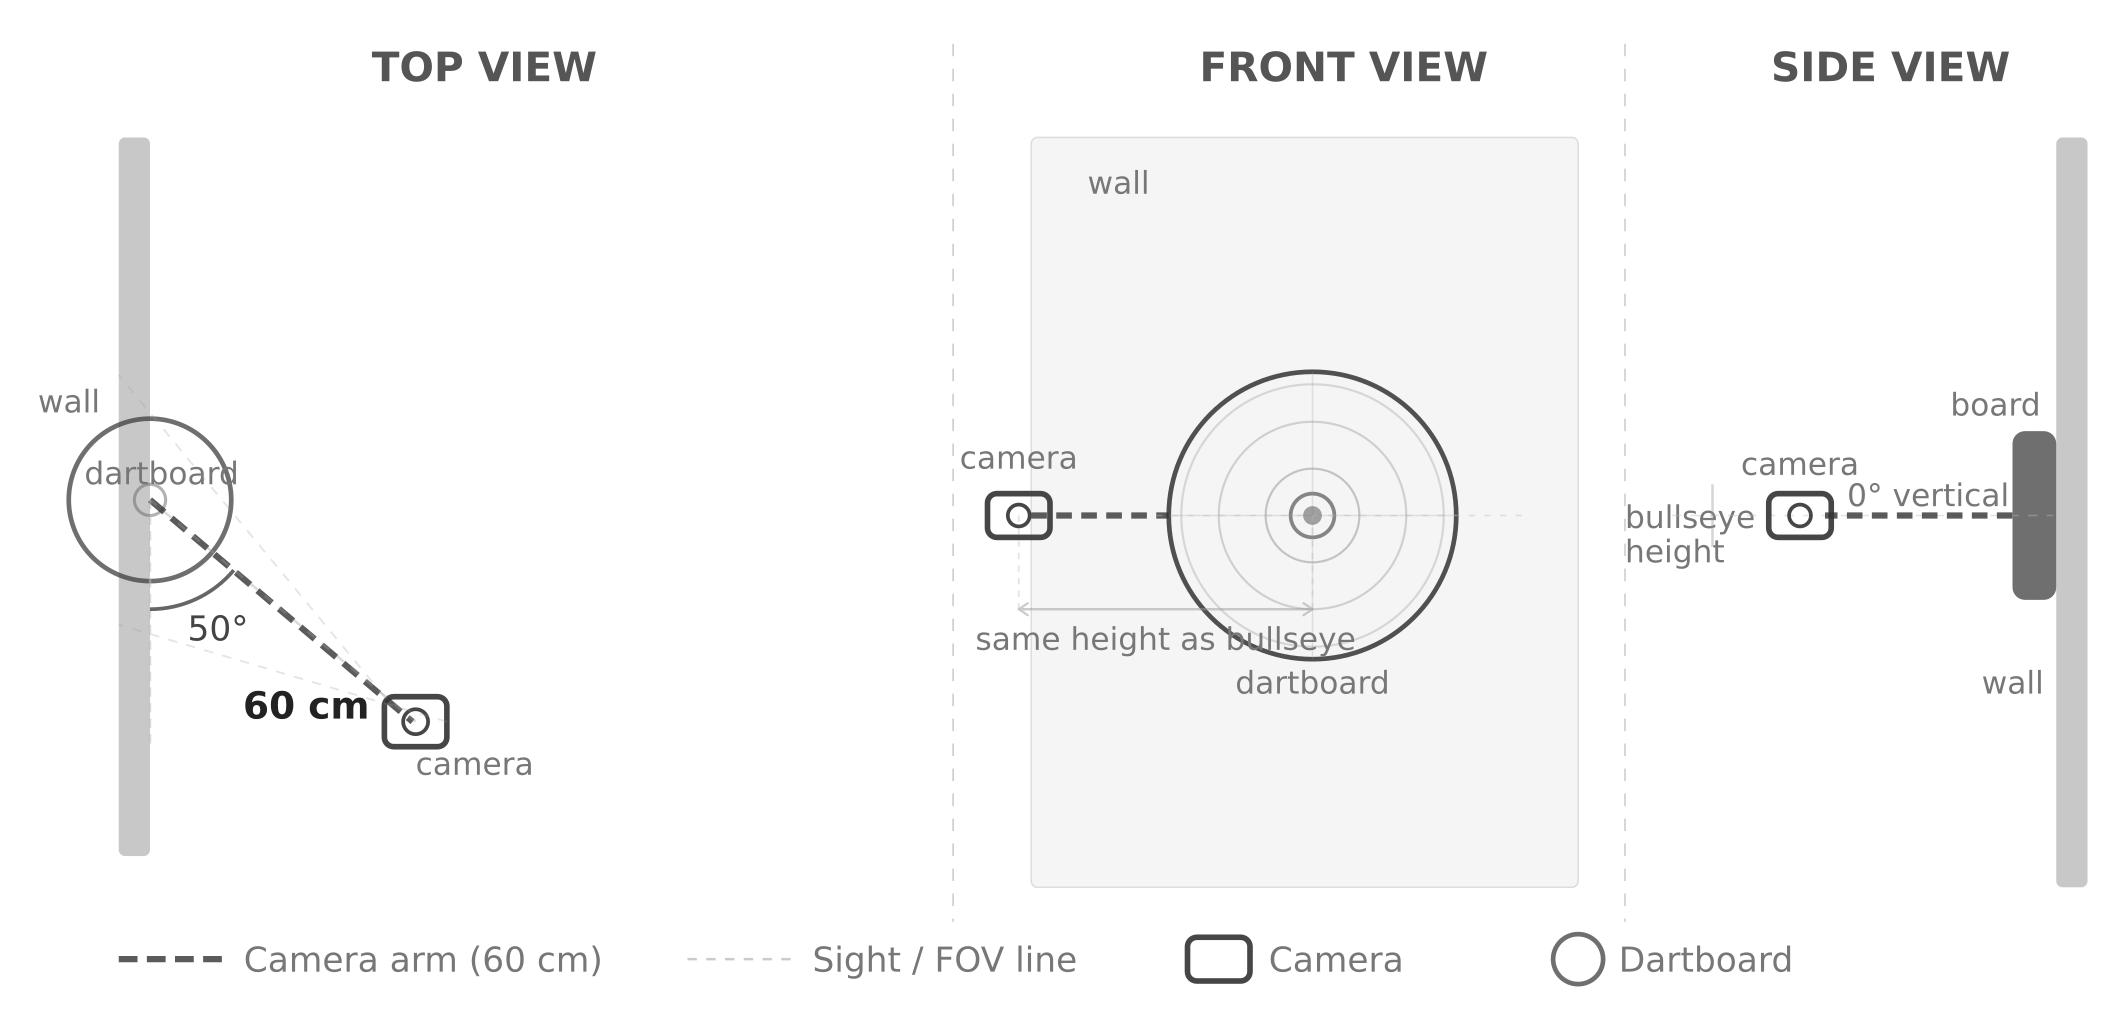
\includegraphics[width=0.9\linewidth]{pics/camera_setup.png}
	\caption{Conceptual sketch of the evaluation setup geometry (camera angle and distance).}
	\label{fig:evaluation_setup_placeholder}
\end{center}


\section{Evaluation Metrics}
\subsection{Hit Position Error}

\subsubsection{Millimeter Deviation}
The system that has been implemented maps the identified tip coordinate location onto the ring sector region in order to classify the hit location, and as such, the most obvious manifestation of the error that the system might make in practice is at the region boundaries. Rather than using the millimeter error value that might be experienced in the system, the evaluation focused more on the ability of the localization system to stay within the correct region for scoring purposes in practice.

Qualitatively, the robustness of the system was observed in the impacts made at the center and the mid sector regions. The most prominent localization uncertainty was observed in the near-boundary throws, where the minor contour shift can cause the tip location to switch from one sector region to another. This behavior can be attributed to the single-camera projection system, where minor distortions and contour variations have the most significant impact near the decision boundaries.


\subsection{Sector Classification Accuracy}

\subsubsection{False Positive Rate}
Across extensive practical throwing sessions (including central hits, boundary-near hits, and out-of-board throws), sector-level classification remained stable enough for recreational play. The quantified accuracy values are reported in Section~\ref{sec:accuracy_consolidation}, where setup-specific outcomes and computed accuracy values are listed in a structured format.

Most misclassifications belonged to one of three categories:

\begin{itemize}
	\item Calibration drift or poor calibration quality, causing systematic sector offset.
	\item Boundary ambiguity when a large contour intersects a sector edge, producing unstable assignment between adjacent sectors.
	\item Vibration-related global motion when the camera mount couples mechanically to the board.
\end{itemize}

The first two categories provided results that, although incorrect, were reasonable within a neighboring area rather than arbitrary data, which further reinforces the proximity of the localization to the actual impact location.

\begin{center}
\captionsetup{type=table,hypcap=false}
	\centering
	\caption{Observed practical outcome classes during evaluation sessions.}
	\label{tab:observed_outcome_classes}
	\begin{tabularx}{\linewidth}{@{}X c X@{}}
		\toprule
		\textbf{Outcome Class} & \textbf{Relative Frequency} & \textbf{Typical Cause} \\
		\midrule
		Correct sector assignment & High & Stable calibration and clean contour extraction \\
		Neighbor-sector misclassification & Medium & Boundary ambiguity and contour edge expansion \\
		Missed hit event & Low to Medium & Camera vibration or insufficient stable post-impact contour \\
		Correctly ignored non-hit event & Medium & Out-of-bounds throw or no persistent board impact \\
		\bottomrule
	\end{tabularx}
\end{center}

\section{Accuracy Consolidation}\label{sec:accuracy_consolidation}

Accuracy is reported at sector level and is based on labeled throws from the evaluation session described in Table~\ref{tab:evaluation_setup_sheet}. Camera placement constraints that influence classification stability are discussed in Section~\ref{subsec:eval_camera_setup}.

For each setup, accuracy is calculated as:

\[
\mathrm{Accuracy} = \frac{N_{\mathrm{correct}}}{N_{\mathrm{total}}} \cdot 100\%
\]

\vspace{\baselineskip}


\subsection{Setup A: Measured Outcomes}

\begin{center}
\captionsetup{type=table,hypcap=false}
	\centering
	\caption{Outcome counts for Setup A.}
	\label{tab:accuracy_setup_a_outcomes}
	\begin{tabularx}{\linewidth}{@{}X c X@{}}
		\toprule
		\textbf{Outcome Category} & \textbf{Count} & \textbf{Interpretation} \\
		\midrule
		Correctly detected & 43 & Correct sector classification \\
		Wrong edge cases & 7 & Dart tip not correctly localized or poorly calibrated \\
		Occluded by another dart & 2 & Visibility limitation due to overlap \\
		Not detected because of motion & 3 & Motion-related detection failure \\
		\midrule
		\textbf{Total throws} & \textbf{55} & Sum of all outcome categories \\
		\bottomrule
	\end{tabularx}
\end{center}

\vspace{\baselineskip}


\noindent \textbf{Computed real accuracy (Setup A):}
\[
\frac{43}{55} \cdot 100\% = 78.2\%
\]

\vspace{\baselineskip}


\subsection{Setup B: Alternative Setup}

\begin{center}
\captionsetup{type=table,hypcap=false}
	\centering
	\caption{Setup B specification sheet.}
	\label{tab:accuracy_setup_b_spec}
	\begin{tabularx}{\linewidth}{@{}X X@{}}
		\toprule
		\textbf{Parameter} & \textbf{Value} \\
		\midrule
		Camera model & TRUST EXIS Webcam \\
		Resolution & $640 \times 480$ \\
		FPS during test & 24 \\
		Camera angle & $45^{\circ}$ \\
		Camera distance & 65 cm \\
		Lighting & Same ring light \\
		\bottomrule
	\end{tabularx}
\end{center}

\vspace{\baselineskip}

\begin{center}
\captionsetup{type=table,hypcap=false}
	\centering
	\caption{Outcome counts for Setup B.}
	\label{tab:accuracy_setup_b_outcomes}
	\begin{tabularx}{\linewidth}{@{}X c X@{}}
		\toprule
		\textbf{Outcome Category} & \textbf{Count} & \textbf{Interpretation} \\
		\midrule
		Correctly detected & 29 & Correct sector classification \\
		Wrong edge cases & 7 & Dart tip not detected due to limited resolution \\
		Occluded by another dart & 2 & Visibility limitation due to overlap \\
		Not detected because of motion & 10 & Camera mount too unstable \\
		\midrule
		\textbf{Total throws} & \textbf{48} & Sum of all outcome categories \\
		\bottomrule
	\end{tabularx}
\end{center}

\vspace{\baselineskip}

\noindent \textbf{Computed real accuracy (Setup B):}
\[
\frac{29}{48} \cdot 100\% = 60.4\%
\]

\vspace{\baselineskip}

\begin{center}
\captionsetup{type=table,hypcap=false}
	\centering
	\caption{Overall accuracy summary across both setups.}
	\label{tab:accuracy_overall_summary}
	\begin{tabularx}{\linewidth}{@{}X c c c@{}}
		\toprule
		\textbf{Scope} & \textbf{Total Throws} & \textbf{Correct} & \textbf{Computed Accuracy (\%)} \\
		\midrule
		Setup A & 55 & 43 & 78.2 \\
		Setup B & 48 & 29 & 60.4 \\
		\textbf{Combined} & \textbf{103} & \textbf{72} & \textbf{70} \\
		\bottomrule
	\end{tabularx}
\end{center}

\section{Edge Case Analysis}

\subsection{Bounce-Outs}
It is not possible to detect these with the current pipeline. The detector assumes that a valid throw results in a newly static object on the board. If a dart bounces off a metal area or touches a dart and then is thrown off, then no final static contour exists, so it is not considered a valid dart.

This is a known methodological limitation as opposed to a programming error. The development of a proper bounce-out detector would require further event modeling, sound/vibration detection, or multi-angle verification.

\subsection{Occluded Darts}
Extreme cases of occlusion were rare in the given board configuration but are relevant in practical environments. If a new dart is thrown into an area close to an already embedded dart, contour union can reduce dart-tip separability. The merged-contour technique currently used is a significant enhancement to increase robustness against fragmented dart contours. However, it can also cause ambiguity between densely grouped darts.

From an empirical standpoint, it was determined that these types of situations were most likely to cause issues with shots landing in near-adjacent segment areas rapidly fired in succession.

\subsection{Motion Blur and Shadows}
Given a 26 FPS rate and ring light illumination, motion blur was not a significant factor in error rates, as the final state is stationary to register a point. However, sudden changes to global illumination or cast shadows can potentially cause issues with threshold determination.

The ring light installation was a significant factor in minimizing potential issues. The few errors that occurred were due to camera vibrations.

\begin{center}
\captionsetup{type=figure,hypcap=false}
	\centering
	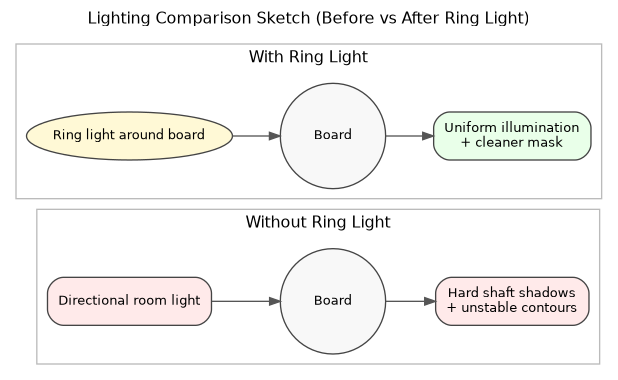
\includegraphics[width=0.95\linewidth]{pics/generated/lighting_comparison_sketch.png}
	\caption{Conceptual before/after sketch of lighting impact on shadow behavior and contour stability.}
	\label{fig:lighting_comparison_placeholder}
\end{center}

\section{Experimental Results}

\subsection{Successful Detection Scenarios}
The strongest results were observed in the following scenarios:

\begin{itemize}
	\item Good calibration with stable camera geometry.
	\item Uniform ring-light illumination with minimal cast shadows.
	\item Camera placement that keeps the full board in frame while maximizing board scale.
	\item Angle near the empirically chosen range ($\approx 45^{\circ}$ to $50^{\circ}$), balancing contour clarity and sector readability.
\end{itemize}

Under these conditions, the detector produced stable contour masks and consistent sector assignment across repeated throws.

\subsection{Failure Scenarios}
Observed failures were repeatable and can be grouped as follows:

\begin{itemize}
	\item \textbf{Calibration error:} Incorrect ring/sector alignment shifts classifications into neighboring fields.
	\item \textbf{Boundary ambiguity:} Large or irregular contours exactly on sector borders can flip between adjacent sectors.
	\item \textbf{Bounce-out behavior:} Non-persistent impacts are not represented in the final static frame and are therefore missed.
	\item \textbf{Mount vibration:} If the camera is mechanically coupled to board vibrations, global frame motion causes detector confusion and can suppress valid detections.
\end{itemize}

\subsection{Reproducibility Checklist}

To improve repeatability of future experiments, the following protocol was derived from the final evaluation setup.

\begin{lstlisting}[numbers=left,caption=Minimal reproducibility protocol for future test repetitions, label=lst:evaluation_repro_protocol]
Verify camera mount rigidity and fixed board alignment.
Confirm ring-light operation and remove directional room light hotspots.
Re-run calibration and save configuration before test session.
Execute mixed throw set: center, near-edge, out-of-bounds, rapid succession.
Log each mismatch under one of the defined failure categories.
Re-test after any parameter adjustment to detect regressions.
\end{lstlisting}

\begin{center}
\captionsetup{type=table,hypcap=false}
	\centering
	\caption{Failure taxonomy used for structured error logging.}
	\label{tab:failure_taxonomy}
	\begin{tabularx}{\linewidth}{@{}X X@{}}
		\toprule
		\textbf{Category} & \textbf{Operational Description} \\
		\midrule
		Calibration error & Sector mapping offset due to inaccurate board reference alignment \\
		Boundary ambiguity & Neighbor-sector flip for impacts exactly on ring/sector borders \\
		Bounce-out limitation & No persistent contour remains after non-sticking impact \\
		Vibration-induced instability & Mount/board coupling causes global frame motion and detector overload \\
		\bottomrule
	\end{tabularx}
\end{center}